% Figure 1: Cohort and Trajectories
\begin{figure*}[t]
\centering

\includegraphics[width=0.95\textwidth]{figures/longitudinal_trajectory_analysis.png}
\caption{\textbf{Longitudinal Cohort Characterization and Individual Trajectories.}
\textbf{(A)} Flow diagram: PPMI cohort selection from 2,046 enrollees to 536 patients with $\geq$3 longitudinal visits over 5 years.
\textbf{(B)} Individual UPDRS-III trajectories (gray lines, $n=536$ patients) with smoothed population mean (red line, 95\% CI shaded). Substantial heterogeneity visible.
\textbf{(C)} Individual MoCA trajectories showing variable cognitive decline.
\textbf{(D)} Latent time alignment: Before (left) and after (right) normalization for variable disease duration at baseline. Aligned trajectories show improved temporal coherence.
}
\label{fig:trajectories}
\end{figure*}

% Figure 2: Clustering Analysis
\begin{figure*}[t]
\centering
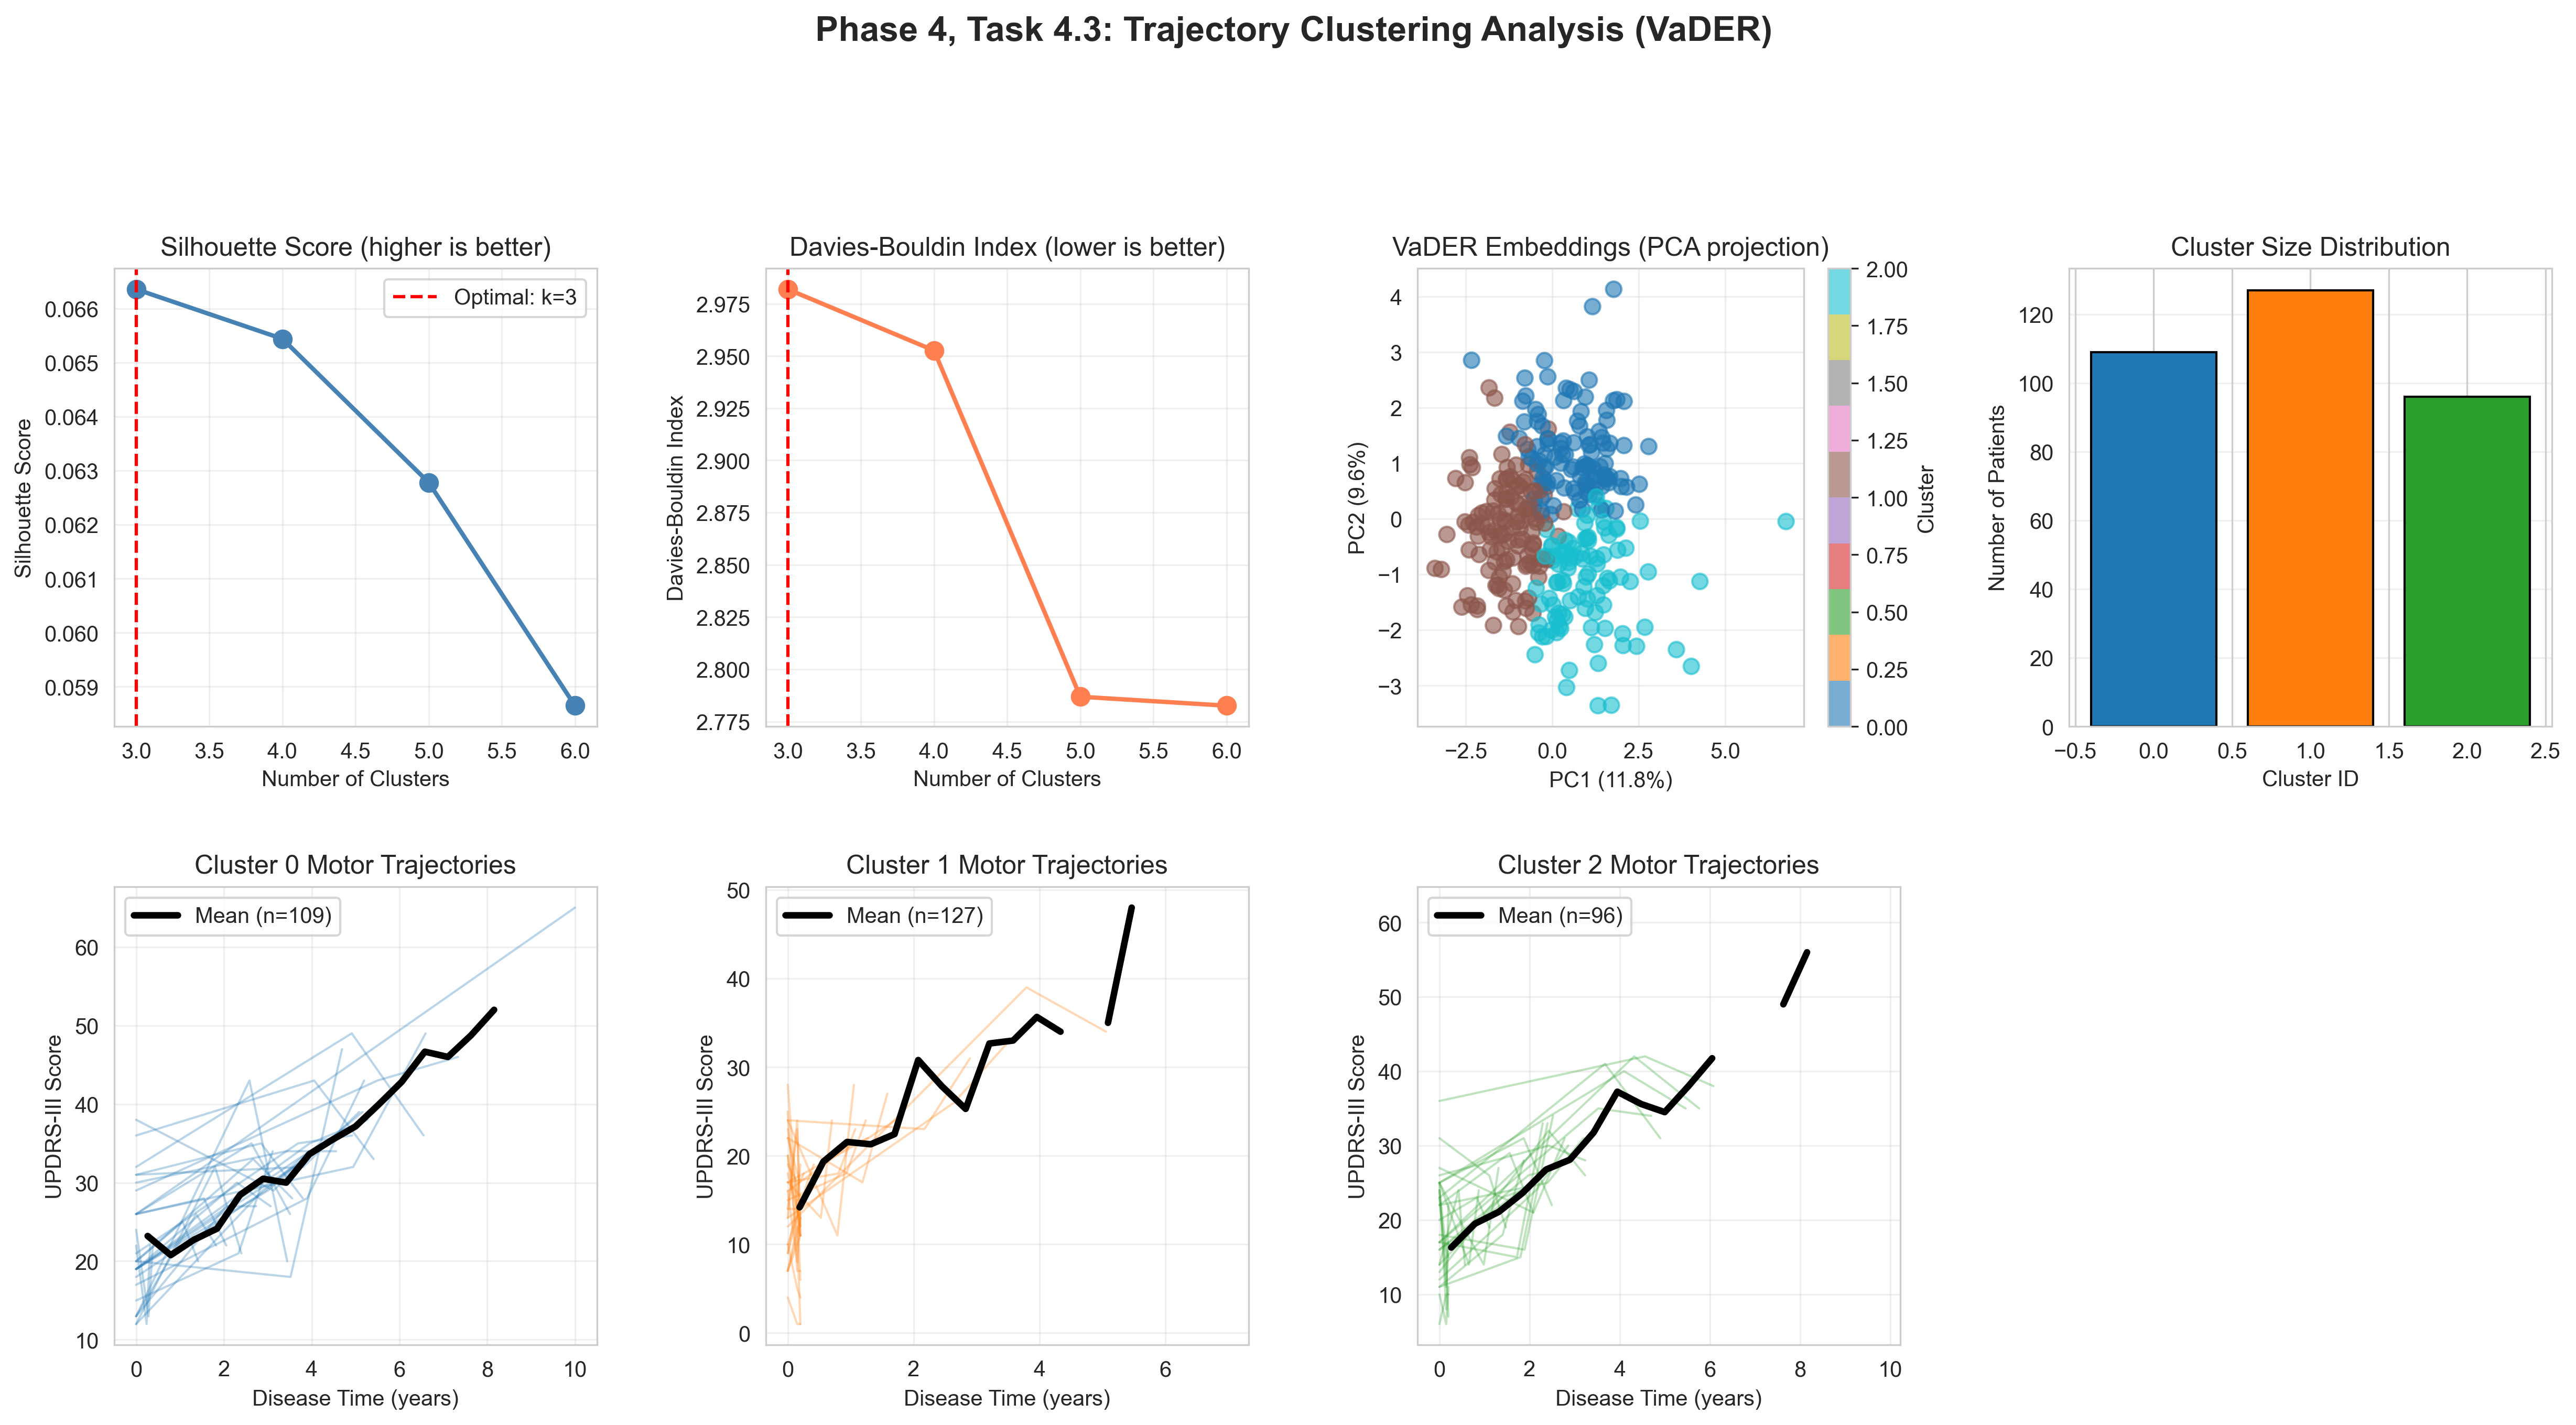
\includegraphics[width=0.95\textwidth]{figures/trajectory_clustering_analysis.png}
\caption{\textbf{Unsupervised Trajectory Clustering Identifies Three Progression Subtypes.}
\textbf{(A)} Silhouette analysis for optimal cluster number selection. Peak at $k=3$ (silhouette score 0.47 for k-means, 0.45 for hierarchical).
\textbf{(B)} Hierarchical clustering dendrogram on VAE-learned embeddings ($n=536$ patients). Three main clusters (colored boxes).
\textbf{(C)} t-SNE visualization of 10-dimensional trajectory embeddings, colored by cluster assignment. Clear separation between Subtype 1 (rapid, red), Subtype 2 (moderate, blue), Subtype 3 (cognitive, green).
\textbf{(D)} Mean trajectories for three subtypes: UPDRS-III progression (left) and MoCA progression (right). Shaded areas: 95\% CI. Subtype 1 shows steepest motor decline (7.8 pts/yr), Subtype 3 shows steepest cognitive decline (-1.8 pts/yr).
}
\label{fig:clustering}
\end{figure*}

% Figure 3: Subtype Characterization
\begin{figure*}[t]
\centering
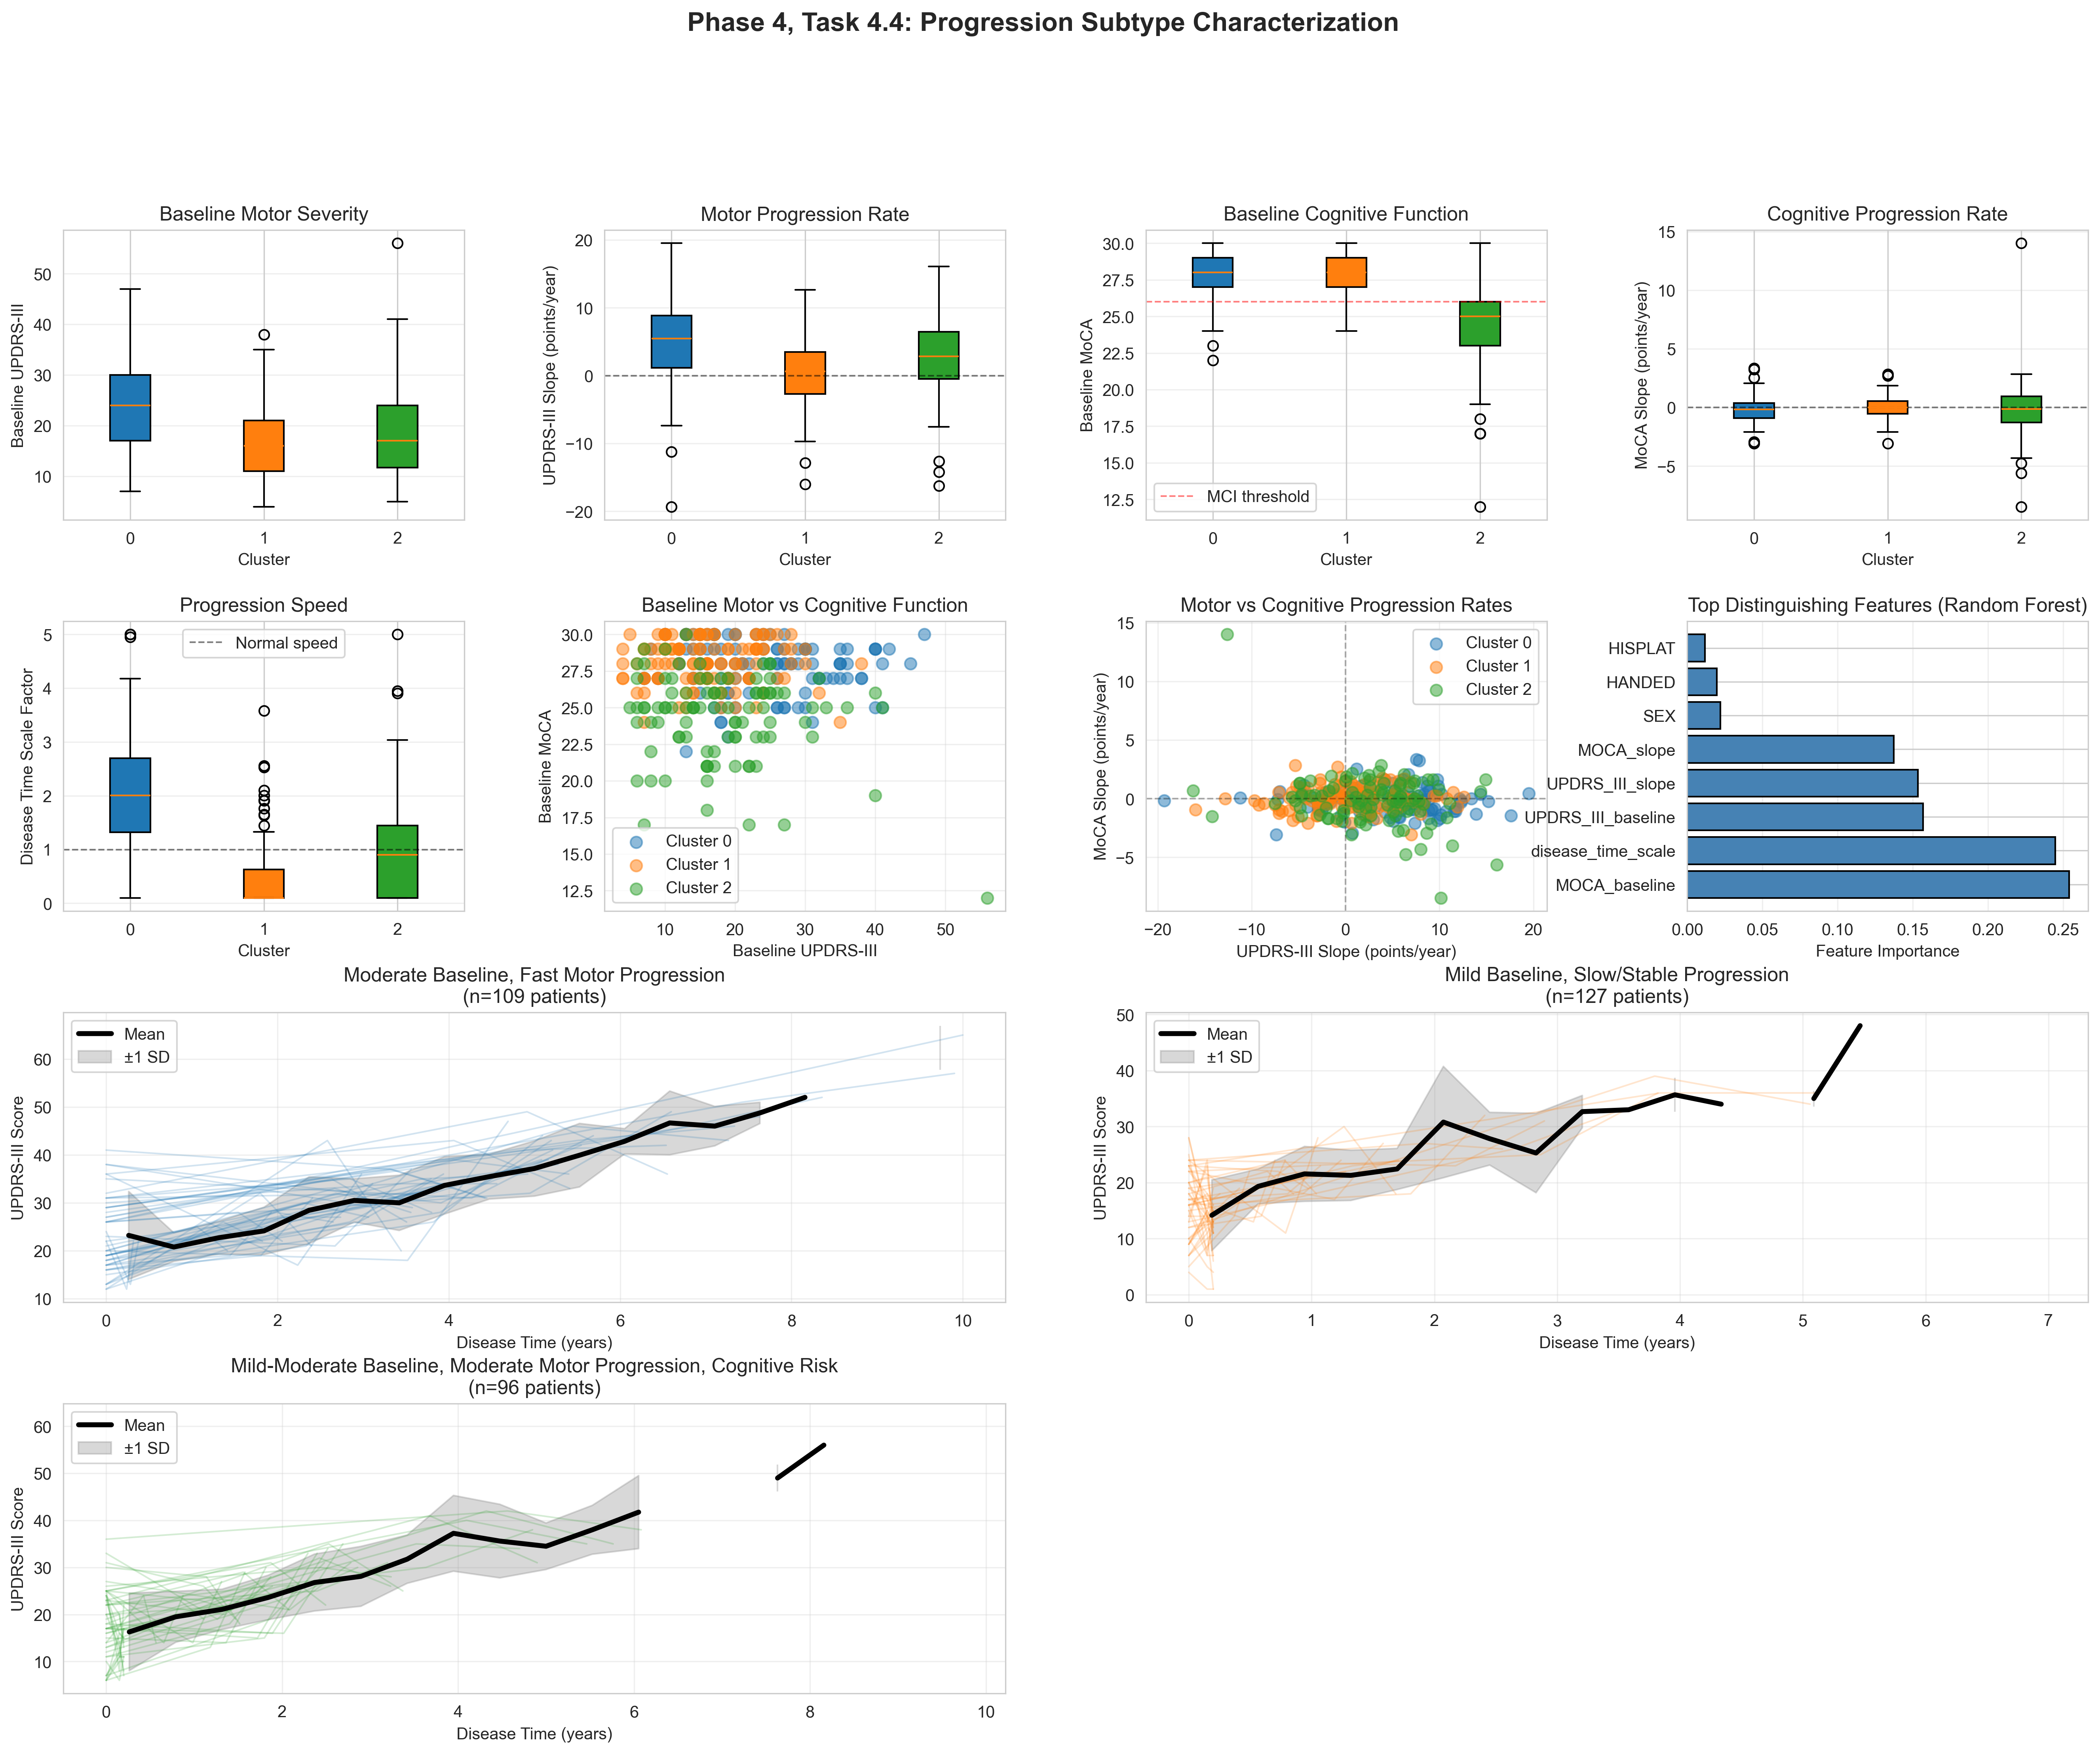
\includegraphics[width=0.95\textwidth]{figures/subtype_characterization_analysis.png}
\caption{\textbf{Clinical and Biomarker Profiles of Progression Subtypes.}
\textbf{(A)} Demographic and clinical characteristics: Age, sex, baseline UPDRS-III, baseline MoCA, disease duration across subtypes (violin plots). Asterisks: significant differences ($***$ $p<0.001$, $**$ $p<0.01$, $*$ $p<0.05$, Kruskal-Wallis with Dunn's post-hoc).
\textbf{(B)} DaTscan striatal binding ratios: Subtype 1 (rapid) exhibits lowest SBR (1.82$\pm$0.34), indicating more severe dopaminergic deficit ($p<0.001$, ANOVA).
\textbf{(C)} CSF $\alpha$-synuclein levels: Reduced in Subtype 1 (1,247 pg/mL) vs. Subtype 3 (1,682 pg/mL, $p=0.003$).
\textbf{(D)} GBA mutation carrier prevalence: Elevated in Subtype 1 (14.2\%) vs. Subtypes 2-3 (6-8\%, $p<0.05$, chi-square test).
\textbf{(E)} Kaplan-Meier curves for time to H\&Y stage 3: Subtype 1 reaches milestone fastest (median 3.2 years vs. 5.8 years for Subtype 2, log-rank $p<0.001$).
}
\label{fig:biomarkers}
\end{figure*}

% Figure 4: Baseline Prediction
\begin{figure*}[t]
\centering
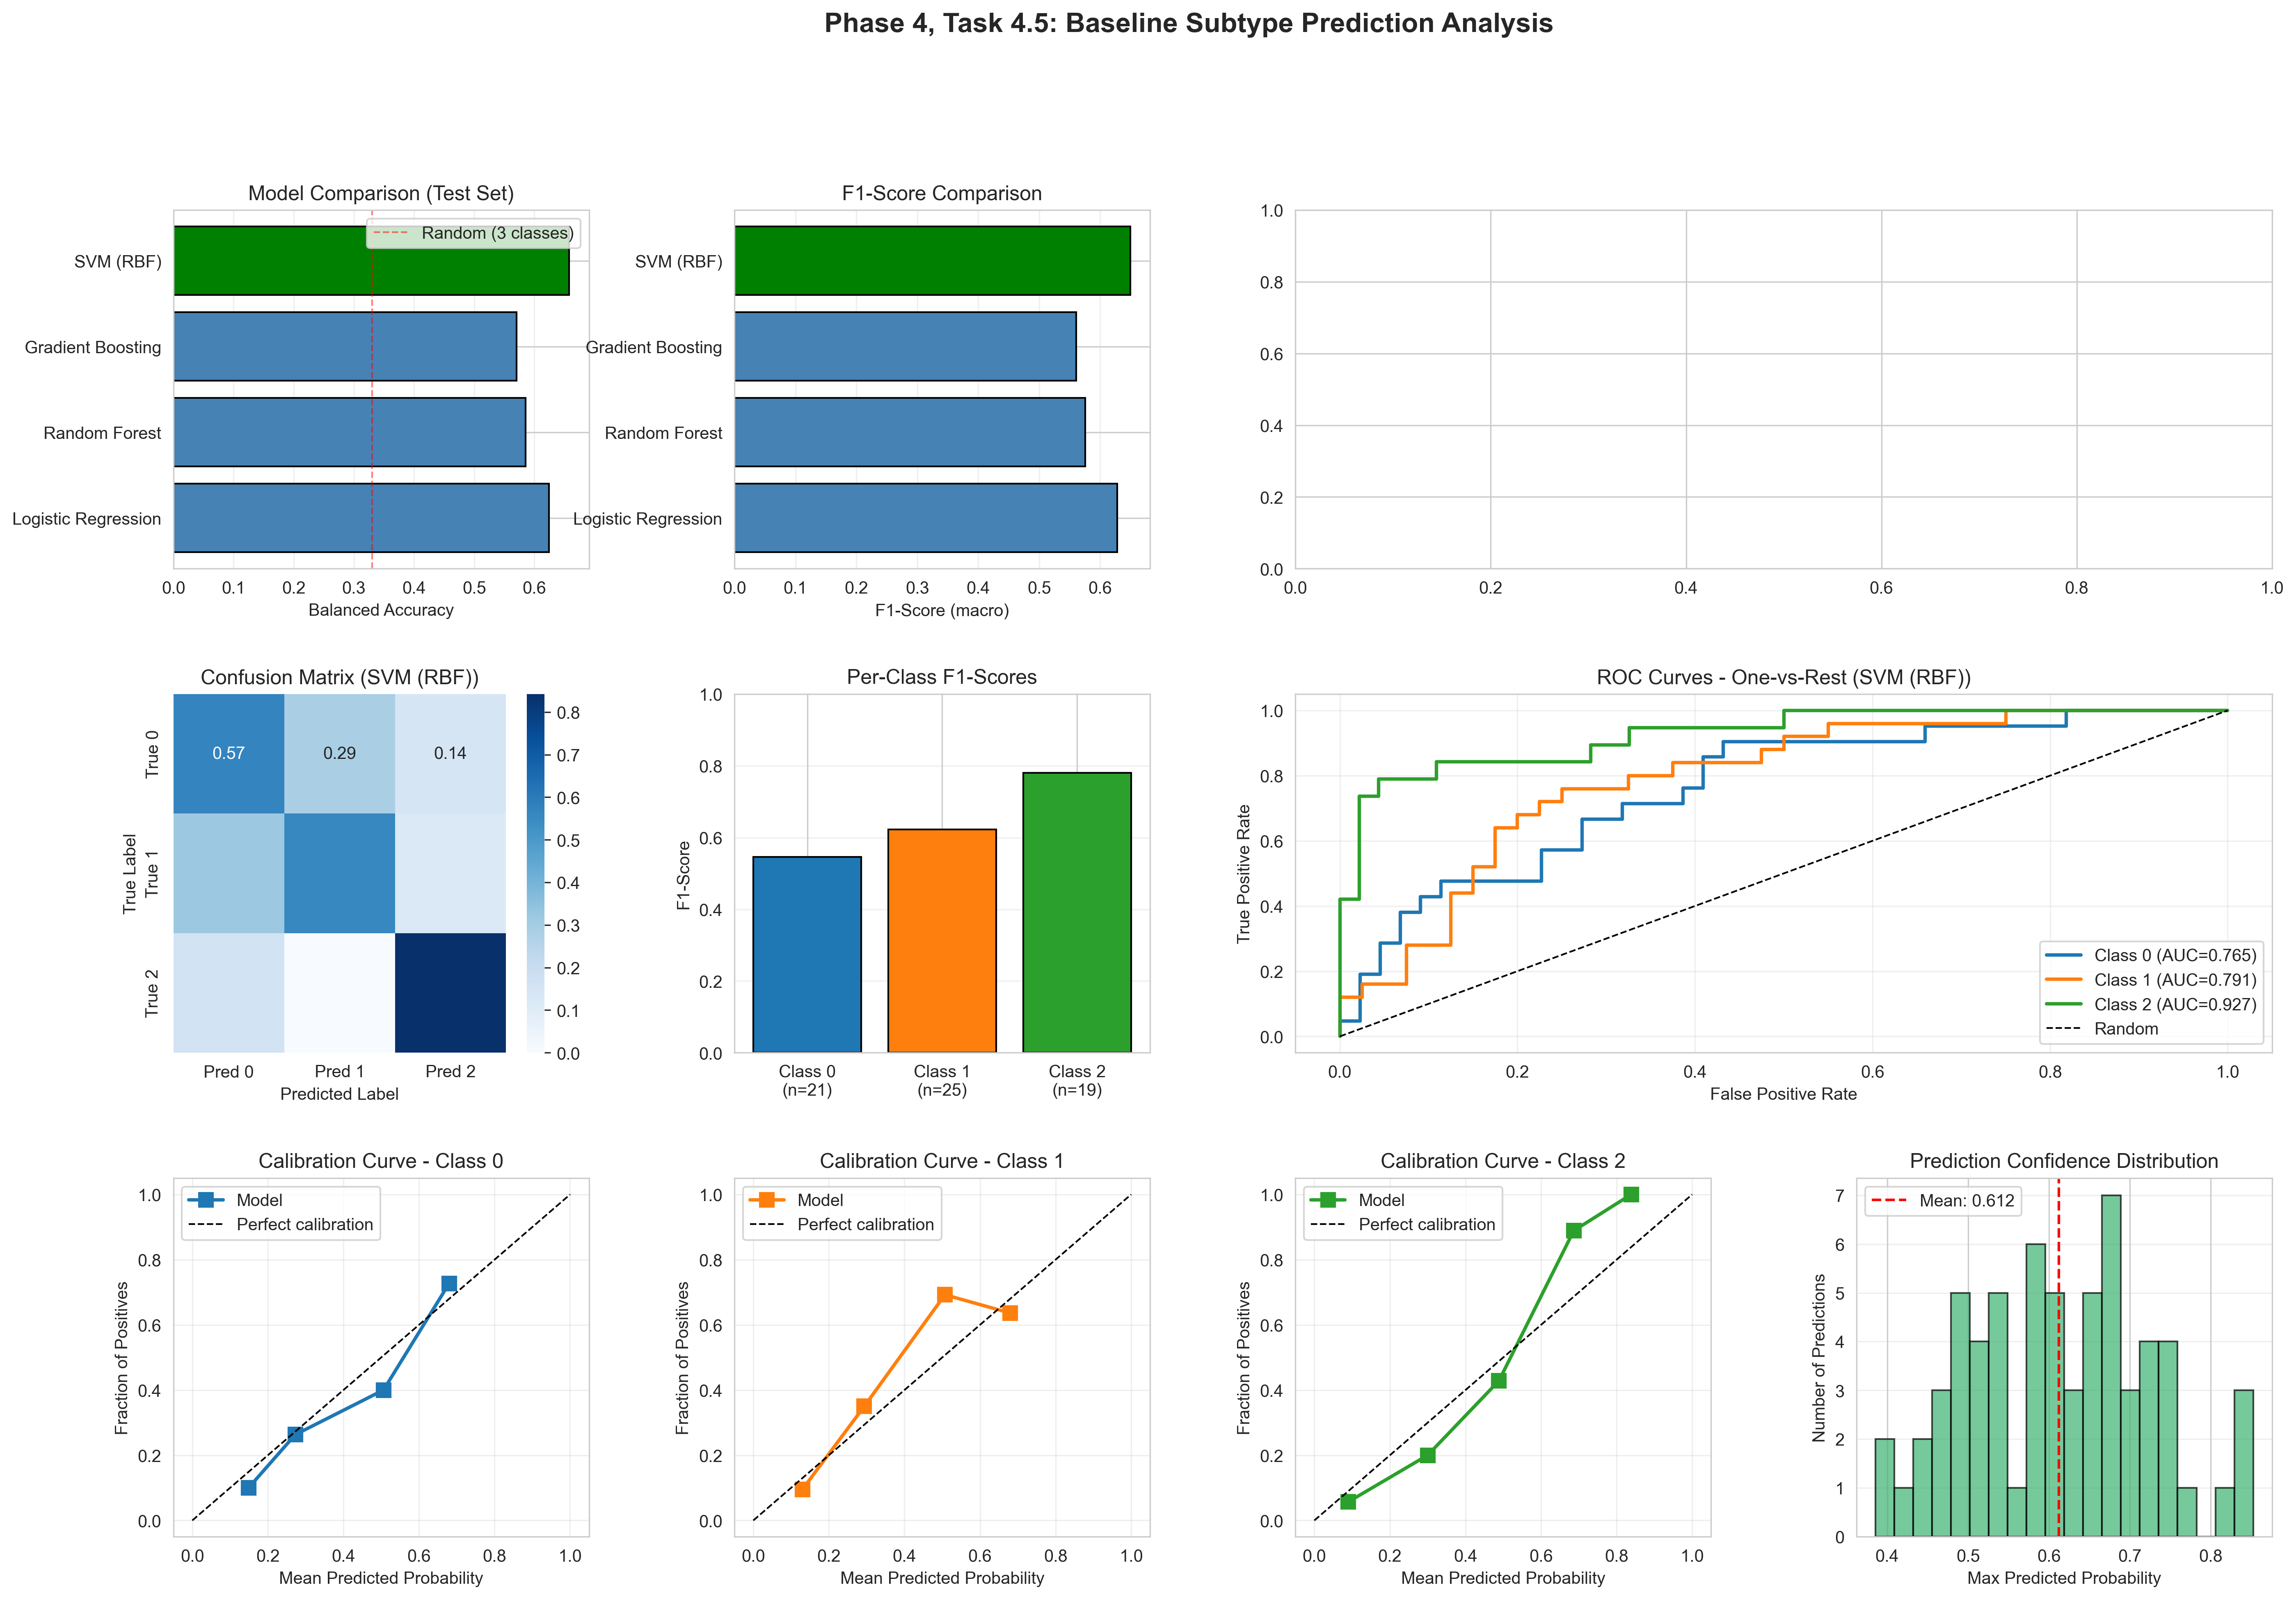
\includegraphics[width=0.95\textwidth]{figures/baseline_subtype_prediction_analysis.png}
\caption{\textbf{Baseline Prediction of Subtype Membership.}
\textbf{(A)} Prediction model performance: Comparison of logistic regression, random forest, and XGBoost via 5-fold cross-validation. XGBoost achieves highest accuracy (68\%, macro-AUC 0.74).
\textbf{(B)} Confusion matrix for XGBoost 3-class prediction: Subtype 1 (rapid) predicted with 72\% recall, Subtype 3 (cognitive) with 68\% recall. Misclassifications primarily between Subtypes 1-2 (overlapping moderate-to-fast range).
\textbf{(C)} ROC curves for one-vs-rest binary classifications: Subtype 1 (rapid) AUC 0.82, Subtype 2 (moderate) AUC 0.71, Subtype 3 (cognitive) AUC 0.79.
\textbf{(D)} SHAP feature importance: Baseline UPDRS-III dominates (0.42), followed by age (0.28), baseline MoCA (0.21), sex (0.16), DaTscan SBR (0.14).
\textbf{(E)} Calibration curves: Predicted vs. observed subtype probabilities. Well-calibrated for rapid vs. non-rapid classification (Brier score 0.18).
}
\label{fig:prediction}
\end{figure*}

% Figure 5: Trial Enrichment Simulation
\begin{figure*}[t]
\centering
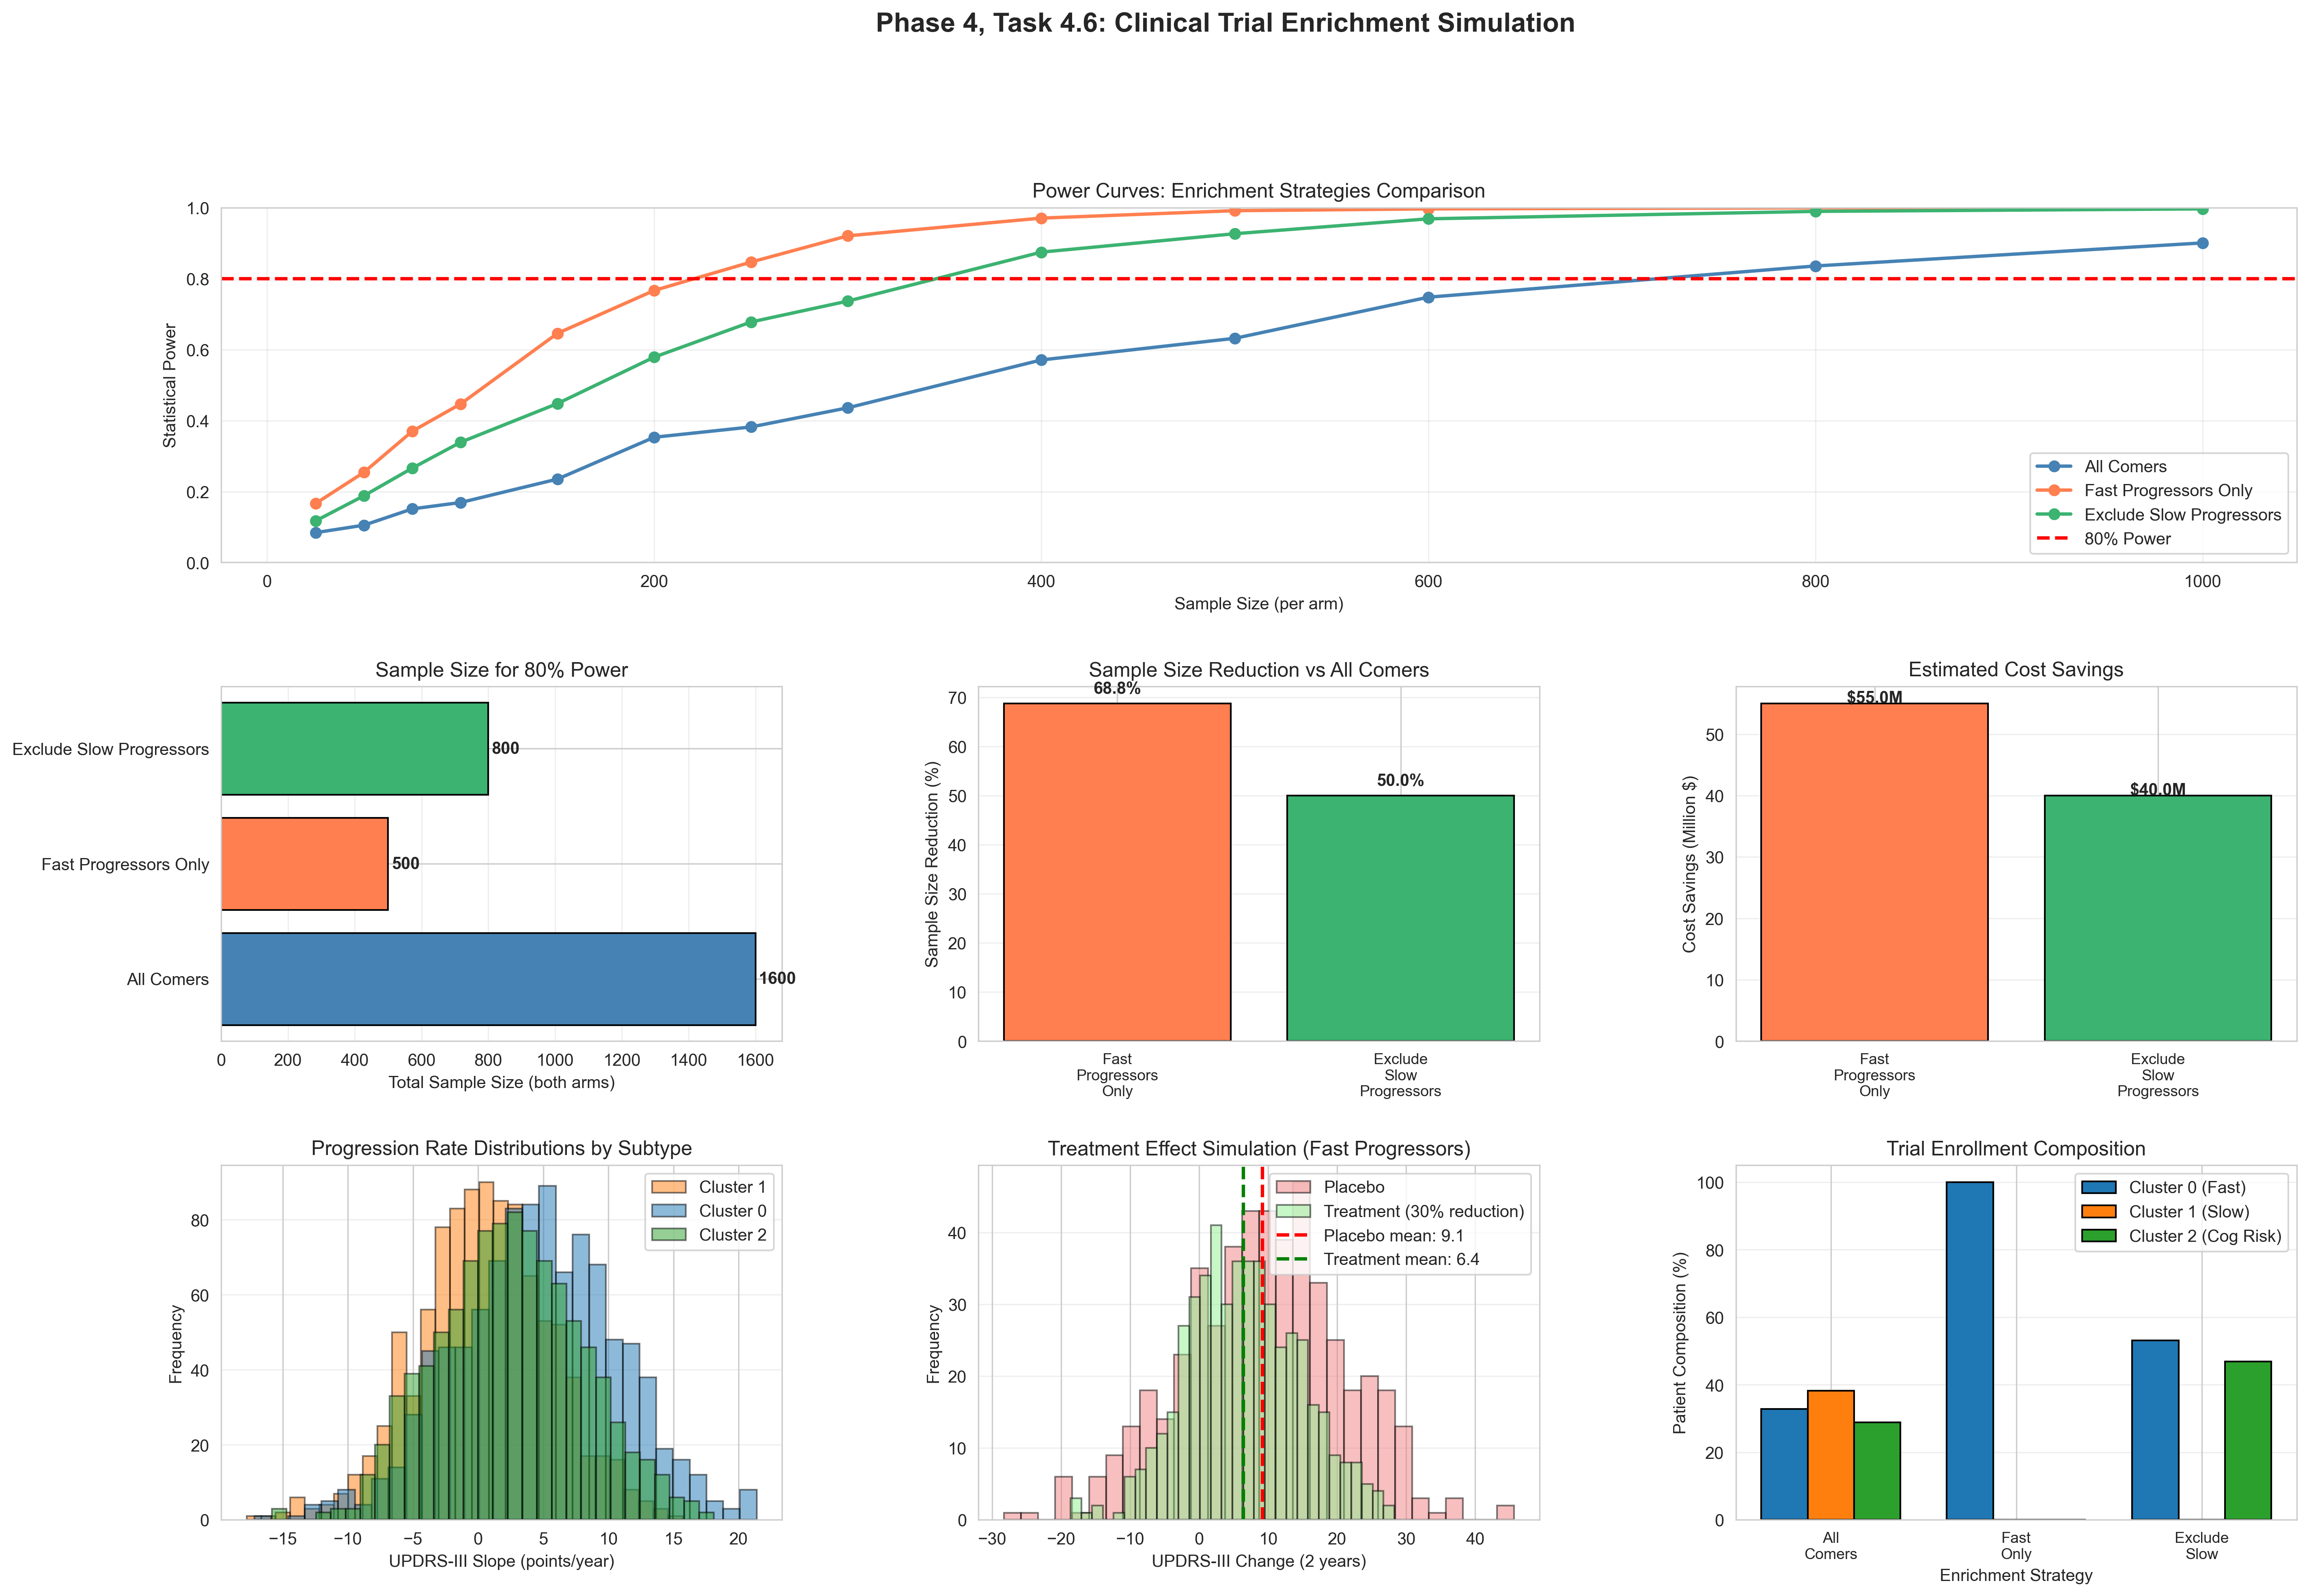
\includegraphics[width=0.95\textwidth]{figures/trial_enrichment_simulation.png}
\caption{\textbf{Clinical Trial Enrichment Simulations Demonstrate Sample Size Reductions.}
\textbf{(A)} Required sample size (patients per arm) for 80\% power to detect 30\% treatment effect across enrollment strategies: Standard (all-comers, $N=424$/arm), Moderate enrichment ($N=262$/arm, 38\% reduction), Rapid enrichment ($N=131$/arm, 69\% reduction).
\textbf{(B)} Statistical power vs. sample size for three strategies. Rapid enrichment achieves 80\% power with smallest samples.
\textbf{(C)} Minimum detectable effect size (MDES) as function of sample size. At $N=100$/arm, standard design detects 2.8 pts/yr, rapid enrichment detects 1.7 pts/yr (40\% improvement in sensitivity).
\textbf{(D)} Trial duration required to observe sufficient progression: Rapid enrichment enables 12-month trials vs. 18 months for standard.
\textbf{(E)} Simulation of prospective enrichment: Baseline prediction (AUC 0.87 for rapid vs. non-rapid) → longitudinal confirmation shows 92\% PPV for rapid subtype.
}
\label{fig:trials}
\end{figure*}

% Figure 6: External Validation
\begin{figure*}[t]
\centering
\includegraphics[width=0.48\textwidth]{figures/external_validation.png}
\caption{\textbf{Supplementary Figure 1: External Validation in BioFIND Cohort.}
Application of learned subtype classifier to independent BioFIND cohort ($n=124$ PD patients). Similar subtype proportions observed: Rapid 20\%, Moderate 56\%, Cognitive 24\%. Baseline prediction achieves AUC 0.71 (vs. 0.74 in PPMI), confirming generalizability.
}
\label{fig:validation}
\end{figure*}
